% todo:
% - přidat obrázek vykreslující autokorelace + popis proč máme 5 iterací
% - odkaz na podkapitoly ve výsledcích (konec kapitoly 6.1)
% - KAPITOLA 6.2 - KVALITA obecně
% - najít zdroj mluvící o využití Hjorthových deskriptorů pro kvalitu signálu
% - aktualizovat obrázek 6.1

\chapter{Využití Hjorthových deskriptorů na odhad TF a kvality signálů}
\label{ch:hjorth}
% Důvody použití Hjorthových deskriptorů pro odhad TF.
% - Metoda nevyžaduje identifikaci systolických vrcholů.
% Argumentace robustností vůči šumu a periodicitou PPG signálu.
% Hjorthovy parametry se běžně používají v EEG (např. pro klasifikaci stavů), ale pro TF z PPG je to méně časté - a tedy inovativní.
V této kapitole je popsán alternativní přístup k odhadu srdeční tepové frekvence (\acs{TF}) z fotopletysmografického signálu (\acs{PPG}), využívající Hjorthovy deskriptory (také označované jako Hjorthovy parametry).
Na rozdíl od standardních metod~\cite{ENIKÖ,Charlton2022,NeuroKit2}, které se opírají o detekci jednotlivých systolických vrcholů a výpočet \acs{IBI}, využívá tento přístup frekvenční vlastnosti analyzovaného signálu.
To je výhodou v případech, kdy je signál poškozen šumem, artefakty, nebo když je kladen důraz na výpočetní náročnost a rychlost algoritmu.

V podkapitole~\ref{sec:hjorth_kvalita} je popsán způsob využití Hjorthových deskriptorů pro hodnocení kvality signálu. % extend

Hjorthovy deskriptory představují trojici příznaků určených z časového průběhu signálu, původně zavedených Hjorthem v~roce 1970 pro kvantitativní popis elektroencefalografických (\acs{EEG}) signálů~\cite{Hjorth1970,Hjorth1973}.
Jedná se o parametry \textit{aktivita} (\(H_0\)), \textit{mobilita} (\(H_1\)) a \textit{komplexita} (\(H_2\)), které odrážejí střední výkon, střední úhlovou frekvenci a šířku pásma.
Jejich výpočet vychází čistě z časové domény a nevyžaduje Fourierovu transformaci.

V dostupné literatuře jsme nenašli studie, které by Hjorthovy deskriptory využívaly k odhadu \acs{TF} z \acs{PPG} signálu.
Proto v této práci navrhujeme a realizujeme nový přístup založený na Hjorthově \textit{mobilitě} (\(H_1\)).
Tu počítáme na filtrovaných a několikanásobně autokorelovaných signálech.
Struktura navrženého algoritmu je znázorněna na Obr.~\ref{fig:hjorth_schemata}.

\begin{figure}[h]
	\centering
	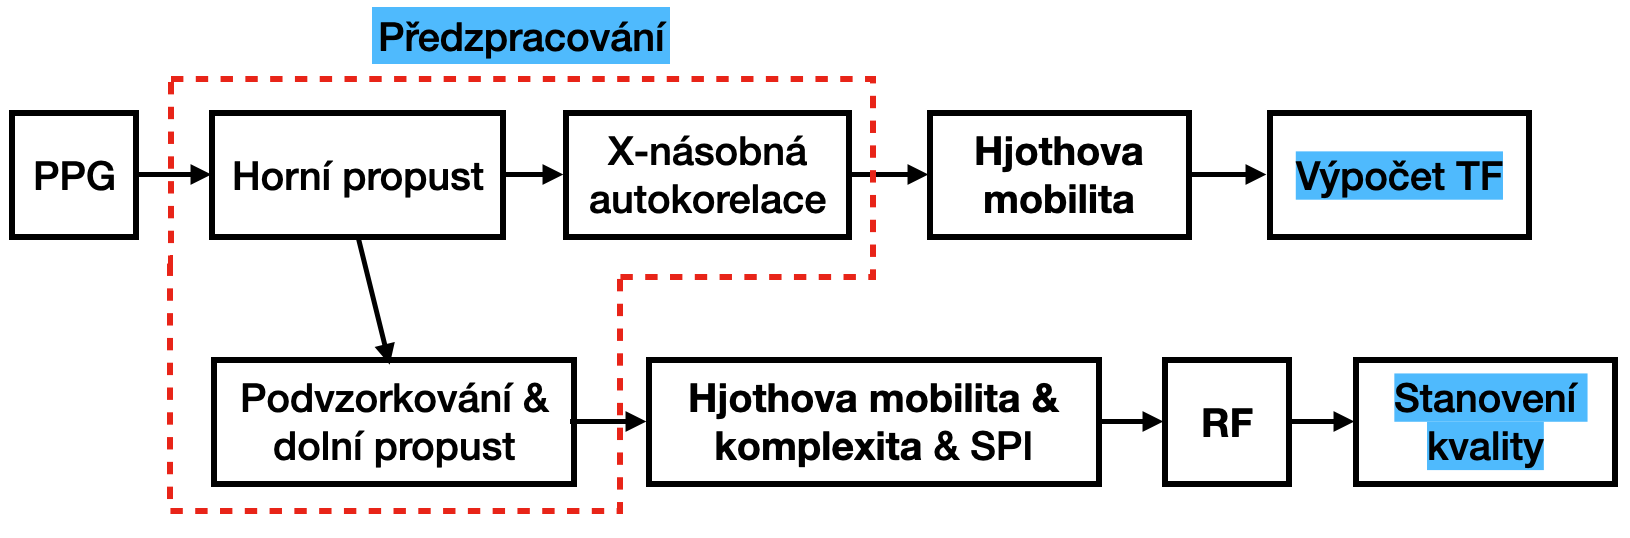
\includegraphics[width=1\textwidth]{./obrazky/hjorth_schema.png} % aktualizovat hodnocení kvality
	\caption[Schéma našeho algorimu, který využívá Hjorthových deskriptorů]{Blokové schéma našeho využití Hjorthových deskriptorů.}
	\label{fig:hjorth_schemata}
\end{figure}

%%%%%%%%%%%%%%%%%%%%%%%%%%%%%%%%%%%%%%%%%%%%%%%%%%%%%%%%%%%%%%%%%%%%%%%%%%%%%%%%
%                                      TEP                                     %
%%%%%%%%%%%%%%%%%%%%%%%%%%%%%%%%%%%%%%%%%%%%%%%%%%%%%%%%%%%%%%%%%%%%%%%%%%%%%%%%
\section{Odhad TF pomocí Hjorthovy mobility}
\label{sec:hjorth_mobilita_tf}
% Načtení signálů z databází probíhá stejně jako u \ref{sec:alg_load}
% Rozdělení signálů je více modulativní, než u \ref{sec:alg_split} pro CapnoBase můžeme použít celý signál nebo libovolný počet oken s maximální délkou odpovídající 10s signálu. Pro BUT PPG (10s signály) to není možné.
Jak již bylo uvedeno, Hjorthova \textit{mobilita} (\( H_1 \)) představuje odhad střední (resp. dominantní) frekvence signálu v časové oblasti a to bez nutnosti výpočtu Fourierovy transformace.

Načtení signálů z databází probíhá stejným způsobem jako u našeho prvního algoritmu, popsaného v podkapitole~\ref{sec:alg_load}.
Odlišný přístup jsme však zvolili při dělení signálů.
Zatímco v předchozím algoritmu jsme signály z \textit{CapnoBase} databáze dělili na minutové úseky, zde si můžeme ve vstupu funkce zvolit libovolný počet úseků, na které signál rozdělíme.
Maximální počet těchto úseků odpovídá situaci, kdy jeden úsek trvá 10~s.
Pokud zbyde po rozdělení signálu část, která je kratší než délka jednoho úseku, tak ji dále nezpracováváme.
Je proto důležité zvolit takové dělení, které minimalizuje délku zahozených úseků.
Alternativou by bylo upravit algoritmus tak, aby zbylé části zpracoval samostatně nebo je přičlenil k předchozímu úseku.
Tím bychom však porovnávali signály různých délek, což by mohlo výsledky zkreslit.

\subsection*{Předzpracování}
\label{sec:predzpracovani}
% Odstranění stejnosměrné složky signálu -> standardizace signálu.
% High-pass filtraci pro odstranění respirační složky.
% Jak fungiuje vícenásobná autokorelace -> cílem je zvýraznění nejdominantnější periodickou složku.
% Grafy autokorelace, původní signál, frekvenční spektrum obou signálů.
% KEEP IN MIND: Nepotlačují se frekvence, ale složky o vyšších/nižších frekvencích.
U analyzovaných signálů jsme provedli standardizaci.
Nejprve jsme odstranili stejnosměrnou (\acs{DC}) složku signálu, tedy jeho střední hodnotu \(\mu\).
Tento krok slouží k centrování signálu kolem nuly, čímž omezíme vliv \acs{DC} složky na výpočet rozptylu signálu.
Druhý krok standardizace je dělení signálu zbaveného hodnoty \(\mu\) jeho směrodatnou odchylkou \(\sigma\).
Rovnice pro standardizaci signálu je následující:
\begin{equation}
	\label{eq:standardizace}
	x[n] = \frac{x[n] - \mu}{\sigma}.
\end{equation}

Následně byl signál filtrován Butterworthovým hornopropustným filtrem čtvrtého řádu s mezní frekvencí 0,5~Hz v obou směrech.
Cílem této filtrace bylo potlačení respirační složky, přičemž prahová frekvence byla zvolena na základě předpokládané minimální hodnoty \acs{TF}, jak je uvedeno v podkapitole~\ref{sec:STF}.

Získaný signál byl dále sedmkrát za sebou autokorelován.
Autokorelace je operace, při které se signál koreluje sám se sebou při různých časových posunech.
Sedminásobná iterace byla zvolena na základě empirického pozorování výsledků na desetisekundových signálech z databáze CapnoBase.
Cílem opakované autokorelace je zvýraznění dominantní periodické složky signálu.
Klasická autokorelační funkce diskrétního signálu \( x[n] \) je definovaná jako:
\begin{equation}
	r_x[m] = \sum_{n=0}^{N-m-1} x[n] \cdot x[n+m],
\end{equation}
kde \( N \) je délka signálu a \( m \) je zpoždění.
Výpočet probíhal ve frekvenční oblasti pomocí rychlé Fourierovy transformace, čímž se snížila výpočetní náročnost na~\(O(i \cdot N \log N)\), kde~\(i\) je počet iterací autokorelace.
Bez použití \acs{FFT} by byla složitost \(O(N^2)\).

Po každé iteraci autokorelace byl signál převeden do rozsahu~\([-1, 1]\) pomocí normalizace podle maximální absolutní hodnoty:
\begin{equation}
	\hat{x}[n] = \frac{x[n]}{\max |x[n]|}.
\end{equation}
Tato normalizace byla nezbytná, protože iterovaná autokorelace způsobuje exponenciální nárůst hodnot, což by vedlo k numerické nestabilitě a zkreslení výpočtu Hjorthových parametrů.

Opakovanou autokorelací dochází ke zvýšení spektrální ostrosti pro dominantní frekvenční složku, což jsme vyhodnotili jako žádoucí pro náš účel.

Porovnání spektra signálu před a po iterované autokorelaci je znázorněno na Obr.~\ref{fig:hjorth_predzpracovani}.
Horní část grafu zobrazuje časové průběhy původního, filtrovaného a autokorelovaného signálu, spodní část pak odpovídající spektra získaná pomocí rychlé Fourierovy transformace.
Amplitudové spektrum bylo vypočteno výhradně pro účely vizualizace a nefiguruje v samotném výpočtu Hjorthových parametrů.
Pro účely porovnání byla všechna spektra převedena na relativní jednotky pomocí normalizace vůči maximální hodnotě amplitudy daného signálu.

\paragraph{}
U běžných \acs{PPG} signálu odpovídají periodické složky systolickým fázím, diastolickým fázím a respiračním složkám.
Pro potlačení respiračních složek jsme použili hornopropustný filtr a pro potlačení složek diastolických fází jsme použili sedm iterací autokorelace.

\begin{figure}[!th]
	\centering
	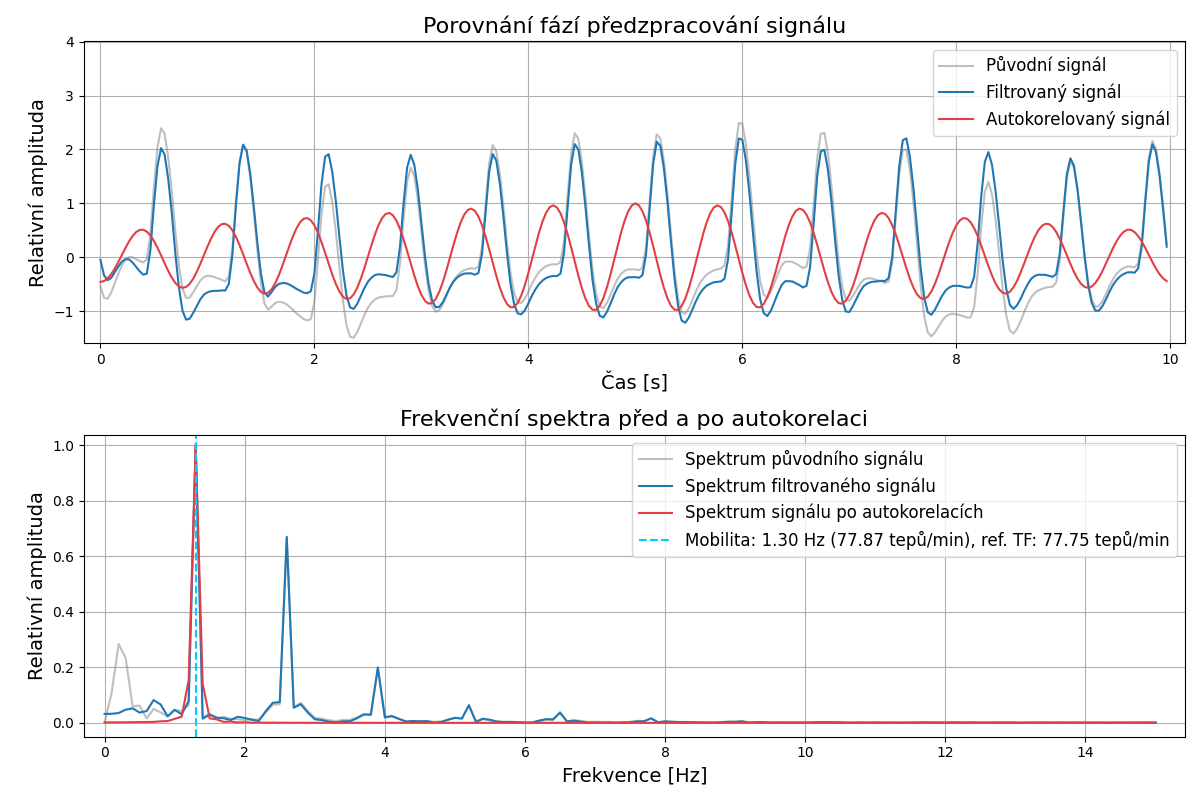
\includegraphics[width=1\textwidth]{./obrazky/hjorth_preprocess.png}
	\caption[Porovnání původního, filtrovaného a autokorelovaného signálu]{Porovnání původního, filtrovaného a autokorelovaného signálu.}
	\label{fig:hjorth_predzpracovani}
\end{figure}

\subsection*{Výpočet TF z mobility}
\label{sec:TF_mobilita}
% Vysvětlení co znamenajá mobilita a jak se počítá -> vzorec.
% Jak se počítá TF z mobility - vzorec.
% první diference = aproximujeme dva body vedle sebe
Po předzpracování signálu jsme vypočítali Hjorthovu mobilitu.
Ta je definována~\cite{Hjorth1970,Geetika2022} jako druhá odmocnina poměru rozptylu první derivace signálu ku rozptylu signálu samotného:
\begin{equation}
	\label{eq:hjorth_mobility}
	H_1 = \sqrt{ \frac{ \mathrm{var}(x[n] - x[n-1]) }{ \mathrm{var}(x[n]) } }
	= \sqrt{ \frac{ \mathrm{var}(x') }{ \mathrm{var}(x) } }
	= \frac{ \sigma_{x'} }{ \sigma_{x} }.
\end{equation}
Jelikož pracujeme v diskrétním prostředí, je derivace aproximována první diferencí.

Rozptyl signálu \( x \) je dán vztahem:
\begin{equation}
	\label{eq:hjorth_var_signal}
	\mathrm{var}(x) = \frac{1}{N} \sum_{n=0}^{N-1} (x[n] - \mu)^2,
\end{equation}
kde \( N \) je délka okna a \( \mu \) je střední hodnota signálu.

Podobně je definován i rozptyl první derivace signálu \( x' \), přičemž první diferenci nelze definovat pro vzorek \( n = 0 \), takže součet začíná až od \( n = 1 \):
\begin{equation}
	\label{eq:hjorth_var_signal_diff}
	\mathrm{var}(x') = \frac{1}{N - 1} \sum_{n=1}^{N-1} (x'[n] - \mu')^2.
\end{equation}

Z hodnoty \( H_1 \) jsme následně odvodili dominantní frekvenci \( f_{dom} \)~[Hz], kterou jsme vynásobili šedesáti, abychom dostali odpovídající hodnotu \acs{TF} v tepech za minutu:
\begin{equation}
	\const{TF}_{\textind{Hjorth}} = 60 \cdot f_{\textind{dom}} = \frac{60 \cdot H_{\textind{1}}}{2\pi}.
\end{equation}
Hodnota dominantní frekvence je graficky znázorněna i písemně zmíněna na Obr.~\ref{fig:hjorth_predzpracovani} společně s odpovídající tepovou frekvencí a referenční hodnotou \acs{TF} z databáze.

\paragraph{}
Přestože mají klasické metody detekce vrcholů~\cite{Elgendi2013} lineární průchod signálem s asymptotickou složitostí \( O(N) \), jejich praktická složitost může být vyšší kvůli víceprůchodovým algoritmům, adaptivním prahům, filtrováním nebo nastavování bloků zájmu (popsané v podkapitole~\ref{sec:blocks}).

Naopak výpočet Hjorthovy mobility má sice po \( i \) iteracích autokorelace (prováděné pomocí \acs{FFT}) složitost \( O(i \cdot N \log N) \), avšak díky své jednoduchosti a absenci větvení může být v praxi rychlejší.

Výsledky odhadu \acs{TF} na základě Hjorthovy mobility jsou diskutovány v kapitole~\ref{ch:vysledky}, přičemž porovnání rychlosti exekuce algoritmů je uvedeno v Tab.~\ref{tab:capnobase_comparison}. % add BUT PPG

%%%%%%%%%%%%%%%%%%%%%%%%%%%%%%%%%%%%%%%%%%%%%%%%%%%%%%%%%%%%%%%%%%%%%%%%%%%%%%%%
%                                    KVALITA                                   %
%%%%%%%%%%%%%%%%%%%%%%%%%%%%%%%%%%%%%%%%%%%%%%%%%%%%%%%%%%%%%%%%%%%%%%%%%%%%%%%%
\section{Hodnocení kvality PPG signálů}
\label{sec:hjorth_kvalita}
% Vysvětlení co znamenajá mobilita a komplexita a jak se počítají -> vzorec.
% - Mobilita_filtr a Komplexita_filtr
% Vysvětlit jak se počítá SPI
% Jaké prahy jsme nastavili pro hodnocení kvality signálu.
Tato podkapitola popisuje metodu automatického hodnocení kvality \acs{PPG} signálů pomocí Hjorthových parametrů s využitím klasifikátoru typu \uv{náhodný les} (\acs{RF}).
Cílem této analýzy je ověřit, zda kombinace tří Hjorthových parametrů — mobility, komplexity a indexu spektrální čistoty (\acs{SPI}) — postačuje k automatické binární klasifikaci \acs{PPG} signálů na základě jejich kvality definované referenčním algoritmem od Orphanidou z knihovny NeuroKit2~\cite{NeuroKit2}.

\subsection*{Segmentace a předzpracování signálů}
\label{subsec:segmentace_predzpracovani}
% KEEP IN MIND: Nepotlačují se frekvence, ale složky o vyšších/nižších frekvencích.
Klasifikátor byl trénován na signálech ze dvou databází: CapnoBase a \acs{BUT PPG}, jejichž záznamy se liší délkou, jak podrobněji popisujeme v kapitole~\ref{chap:databaze}.

Pro zajištění srovnatelnosti Hjorthových deskriptorů mezi oběma databázemi byly signály z CapnoBase rozděleny na nepřekrývající se segmenty o délce 10~s, což odpovídá délce jednotlivých záznamů v databázi \acs{BUT PPG}.
Tato segmentace zároveň přispívá ke konzistenci vstupních dat a zvyšuje přesnost rozhodování jednotlivých stromů klasifikátoru.

Následně byly signály z CapnoBase převzorkovány na vzorkovací frekvenci 30~Hz, aby odpovídaly frekvenci signálů z databáze \acs{BUT PPG}.
Převzorkování bylo realizováno pomocí funkce \texttt{resample} z knihovny \texttt{scipy}, která implementuje Fourierovu interpolaci.
Jelikož tato metoda neobsahuje předběžnou dolnofrekvenční filtraci, mohlo by při přítomnosti vyšších frekvenčních složek dojít k aliasingu.

Abychom tomuto jevu předešli, aplikovali jsme před převzorkováním dolnopropustný filtr typu Butterworth čtvrtého řádu s mezní frekvencí 14~Hz.
Tím jsme potlačili složky nad polovinou cílové vzorkovací frekvence a zachovali pouze spektrum relevantní pro analýzu srdeční činnosti.

Po sjednocení délky a vzorkovací frekvence byly všechny signály standardizovány viz~(\ref{eq:standardizace}).
V souladu s postupem uvedeným v podkapitole~\ref{sec:hjorth_mobilita_tf} jsme dále odstranili nízkofrekvenční složky pod 0,5~Hz.
Zde jsme navíc potlačili i složky nad 3,35~Hz (201 tepům za minutu), čímž jsme omezili spektrum pouze na fyziologicky očekávané rozsahy srdeční frekvence.

\subsection*{Výpočet příznaků pro náhodný les}
\label{subsec:rf_features}
% mobilitu jsme už popsali = eq:hjorth_mobility
% navíc popsat komplexitu a SPI
% komplexita definovaná v Hjorth1970 je ve VUT pojmenována jako "Relativní složitost"
První dva příznaky odpovídají Hjorthovým parametrům, přičemž mobilita (\acs{H_1}) již byla popsána v předchozí podkapitole rovnicí~(\ref{eq:hjorth_mobility}).

Druhý příznak, Hjorthova komplexita (\acs{H_2}), kvantifikuje míru toho, jak se signál v čase odchyluje od harmonického průběhu.
Je definována jako poměr mobility první derivace signálu ku mobilitě samotného signálu~\cite{Hjorth1970,Geetika2022}:
\begin{equation}
	\label{eq:hjorth_complexity}
	H_{2} = \sqrt{ \frac{H_1(x')}{H_1(x)} }
	= \sqrt{ \frac{ \text{var}(x'') / \text{var}(x') }{ \text{var}(x') / \text{var}(x) } }
	= \frac{ \sigma_{x''} \cdot \sigma_{x} }{ \sigma_{x'}^2 } \; [-],
\end{equation}
kde $x$, $x'$, $x''$ jsou signál, jeho první derivace a jeho druhá derivace.
$\sigma_x$ označuje směrodatnou odchylku.
Pro čistě harmonický signál, jako je sinusoida, by vycházelo $H_2 = 1$.
S rostoucím podílem vyšších frekvenčních složek se však signál stává proměnlivějším, a tím vyšší je hodnota \( H_2 \).

Hjorthova komplexita tak slouží jako bezrozměrný ukazatel nepravidelnosti signálu např. při automatickém hodnocení kvality EEG signálů~\cite{Geetika2022}.

Třetím příznakem je index spektrální čistoty (\acs{SPI}), který je definován jako převrácená hodnota komplexity:
\begin{equation}
	\label{eq:hjorth_SPI}
	SPI = \frac{1}{H_2} = \frac{\sigma_{x'}^2}{\sigma_{x''} \cdot \sigma_{x}} \; [-].
\end{equation}

Všechny tři příznaky jsou standardizovány pomocí funkce \texttt{StandardScaler}, aby byl zajištěn jejich jednotný váhový vliv při klasifikaci.

\subsection*{Referenční hodnota kvality}
\label{subsec:referencni_hodnota_kvality}
% Referenčním hodnotám uvedených v BUT PPG nevěříme, proto musíme implementovat Orphanidou výpočet kvality z NeuroKit2 = sami si nastavíme referenční kvalitu signálů

% Po vizuální analýze anotací kvality signálů v databázi BUT PPG bylo zjištěno, že tyto anotace nejsou dostatečně konzistentní (obr.~\ref{fig:orphanidou_vs_db}).
% Z tohoto důvodu jsme jako referenční hodnotu zvolili tzv. Orphanidou index kvality, který je implementován v knihovně NeuroKit2.

% Tento index funguje následovně: z každého 10sekundového signálu jsou nejprve detekovány pulzní vrcholy.
% Poté se z těchto pulzů vytvoří průměrná šablona. Každý jednotlivý puls je následně porovnán s touto šablonou pomocí Pearsonova korelačního koeficientu:

% \begin{equation}
% 	r_i = \frac{\sum_{n=1}^N (x_n - \bar{x})(y_n - \bar{y})}{\sqrt{\sum_{n=1}^N (x_n - \bar{x})^2} \cdot \sqrt{\sum_{n=1}^N (y_n - \bar{y})^2}},
% \end{equation}

% kde $x$ je šablona a $y$ aktuální pulzní vlna.
% Výsledný index kvality $QI$ je pak dán průměrem těchto korelací v rámci jednoho signálu:

% \begin{equation}
% 	QI = \frac{1}{m} \sum_{i=1}^m r_i,
% \end{equation}

% kde $m$ je počet detekovaných pulzů.
% Segment je považován za kvalitní, pokud $QI \ge 0{,}9$.

\subsection*{Náhodný les}
\label{subsec:random_forest}
% Klasifikátor je Random Forest, který je vhodný pro zpracování malého počtu příznaků.
% Vysvětlit jak funguje Random Forest
% Stratifikace = zajištění stejného poměru tříd v trénovací a testovací sadě
Pro odhad kvality signálů byl použit již zmíněný klasifikátor \emph{náhodný les} (\acs{RF}), který tvoří sadu rozhodovacích stromů a kombinuje jejich výstupy hlasováním.
Použili jsme implementaci \texttt{RandomForestClassifier} z knihovny \texttt{scikit-learn}.
Tento algoritmus je vhodný pro úlohy s omezeným počtem příznaků.
Oproti lineárním modelům dokáže zachytit i nelineární vztahy mezi příznaky a je robustní vůči nadměrnému přizpůsobení.

Model byl trénován se základními vstupy: 50 rozhodovacích stromů, maximální hloubka stromu 5 a výběr příznaků pro jednotlivé uzly dle odmocniny z celkového počtu příznaků. % je slovo vstup správně? pro celý text?
Pro zajištění deterministického chování byl vstup náhodné inicializace nastaven na hodnotu \texttt{random\_state = 42}.
Optimalizace všech vstupů byla provedena pomocí metody \texttt{GridSearchCV} z knihovny \texttt{scikit-learn}, která systematicky vybírá nejlepší kombinace z námi předdefinovaných hodnot.

Datová sada byla rozdělena v poměru 60~\% pro trénování a 40~\% pro testování.
Pomocí vstupu \texttt{class\_weight='balanced'} jsme zajistili, že model bude trénován s ohledem na nevyváženost tříd, tedy poměr kvalitních a nekvalitních signálů.

Výhodou \acs{RF} je rovněž možnost stanovit relativní důležitost jednotlivých příznaků na základě jejich vlivu na rozhodování stromů, což přispívá k interpretovatelnosti modelu a transparentnosti výsledků. % fakt?

Pro hodnocení výkonnosti modelu bylo použito pětinásobné křížové ověření.
Hlavní metrikou bylo $F_1$ skóre, které je vhodné zejména pro nevyvážené datové sady, protože zohledňuje jak \acs{PPV}, tak citlivost (\acs{Se}).

Při hodnocení výsledků algoritmů detekující \acs{TF} kde jsme porovnávali odchylky od referenční hodnoty \acs{TF} pro kvalitní a nekvalitní signály.
Hodnoty kvality signálů jsou odvozeny z \dots % buď Orphanidou nebo výsledky náhodného lesa
